\documentclass{ubicomp-ext}
\usepackage{libertine} % for the pretty dark-circle-enclosed numbers
\usepackage{tikz}
\usepackage{float}
\usepackage{listings}
\usepackage{multicol}
\usepackage{color}
\usepackage{minibox}
\usepackage{fancybox}
\usepackage{fontspec}
\usepackage{ifthen}
\newfontfamily{\lstsansserif}[Scale=.7]{Arial}
\newfontfamily{\textlst}{Arial}
\definecolor{Lemon}{HTML}{FFFACD}
\newcounter{lstNoteCounter}
\newcommand{\lnnum}[1]
    {\ifthenelse{#1 =  1}{\libertineGlyph{uni2776}}
    {\ifthenelse{#1 =  2}{\libertineGlyph{uni2777}}
    {\ifthenelse{#1 =  3}{\libertineGlyph{uni2778}}
    {\ifthenelse{#1 =  4}{\libertineGlyph{uni2779}}
    {\ifthenelse{#1 =  5}{\libertineGlyph{uni277A}}
    {\ifthenelse{#1 =  6}{\libertineGlyph{uni277B}}
    {\ifthenelse{#1 =  7}{\libertineGlyph{uni277C}}
    {\ifthenelse{#1 =  8}{\libertineGlyph{uni277D}}
    {\ifthenelse{#1 =  9}{\libertineGlyph{uni277E}}
    {\ifthenelse{#1 = 10}{\libertineGlyph{uni277F}}
    {\ifthenelse{#1 = 11}{\libertineGlyph{uni24EB}}
    {\ifthenelse{#1 = 12}{\libertineGlyph{uni24EC}}
    {\ifthenelse{#1 = 13}{\libertineGlyph{uni24ED}}
    {\ifthenelse{#1 = 14}{\libertineGlyph{uni24EE}}
    {\ifthenelse{#1 = 15}{\libertineGlyph{uni24EF}}
    {\ifthenelse{#1 = 16}{\libertineGlyph{uni24F0}}
    {\ifthenelse{#1 = 17}{\libertineGlyph{uni24F1}}
    {\ifthenelse{#1 = 18}{\libertineGlyph{uni24F2}}
    {\ifthenelse{#1 = 19}{\libertineGlyph{uni24F3}}
    {\ifthenelse{#1 = 20}{\libertineGlyph{uni24F4}}
    {NUM TOO HIGH}}}}}}}}}}}}}}}}}}}}}


\newcommand{\lstref}[1]{\lnnum{\ref{#1}}}

\newcommand{\lstnote}[1] {
\vbox{\llap{{\lnnum{\ref{#1}}}\hskip 1em}}\label{#1}
}

\lstnewenvironment{csource}[1][]
{
 \setcounter{lstNoteCounter}{0}
 \lstset{basicstyle=\lstsansserif, frame=lines, framexleftmargin=0.5em,
            framexrightmargin=0.5em, backgroundcolor=\color{Lemon}, showstringspaces=false, escapeinside={(*@}{@*)}, #1}
}{}
% Please be sure that you have the dependencies (i.e., additional LaTeX packages) to compile this example.

\copyrightinfo{
  Copyright is held by the author/owner(s).\\
  {\emph{UbiComp '13 Adjunct}}, Sept 8-12, 2013, Zurich, Switzerland.\\
  ACM 978-1-4503-2139-6/13/09...\$15.00.
}

\title{Torwads Context-Oriented Programming in Wireless Sensor Networks}

\numberofauthors{8}
% Notice how author names are alternately typesetted to appear ordered in 2-column format;
% i.e., the first 4 autors on the first column and the other 4 auhors on the second column.
% Actually, it's up to you to strictly adhere to this author notation.
\author{
  \vspace{-1.5em} % lisatolles: The abstract heading should start at the time height on the page as the authors names
  \alignauthor{
  	\textbf{First Author}\\
  	\affaddr{AuthorCo, Inc.}\\
  	\affaddr{123 Author Ave.}\\
  	\affaddr{Authortown, PA 54321 USA}\\
  	\email{author1@anotherco.com}
  }\alignauthor{
  	\textbf{Fifth Author}\\
  	\affaddr{AuthorCo, Inc.}\\
  	\affaddr{123 Author Ave.}\\
  	\affaddr{Authortown, PA 54321 USA}\\
  	\email{author5@anotherco.com}
  }
  \vfil
}

% Paper metadata (use plain text, for PDF inclusion and later re-using, if desired)
\def\plaintitle{UbiComp 2013 LaTeX Extended Abstracts Template}
\def\plainauthor{Luis A. Leiva}
\def\plainkeywords{Guides, instructions, author's kit, conference publications}
\def\plaingeneralterms{Documentation, Standardization}

\hypersetup{
  % Your metadata go here
  pdftitle={\plaintitle},
  pdfauthor={\plainauthor},  
  pdfkeywords={\plainkeywords},
  pdfsubject={\plaingeneralterms},
  % Quick access to color overriding:
  %citecolor=black,
  %linkcolor=black,
  %menucolor=black,
  %urlcolor=black,
}

\usepackage{graphicx}   % for EPS use the graphics package instead
\usepackage{balance}    % useful for balancing the last columns
\usepackage{bibspacing} % save vertical space in references


\begin{document}

\maketitle

\begin{abstract}
  We present our ongoing work towards applying the context-oriented
  programming paradigm to wireless sensor networks
  (WSNs). Context---as a representation of the environment where the
  system operates---plays a key role in WSNs. For example, WSN
  applications must often adapt their operation depending on
  environmental data. We argue that promoting a notion of context as a
  first-class citizen in WSN programming facilitates the design and
  implementation of context-dependent functionality. To this end, we
  conceive a context-oriented programming model expressly tailored to
  WSNs, coupled with dedicated language constructs. Unlike the
  existing literature on context-oriented programming, we embed the
  latter within low-level C-like languages that do not rely on
  resource-intensive features such as dynamic memory management. To
  make our design concrete, we describe a context-oriented extension
  of nesC, a widely used WSN programming language, and report on a
  preliminary assessment of our design.

% Programming for embedded systems makes a significant part in the modern software development. Despite the rapid growth of the high-level languages there are still a necessity to use embedded systems. The prime example of this are Wireless Sensor Networks (WSNs). Most of the platforms for them are embedded.

% The main task of WSNs is to monitor the environment. Thus, they are widely applied in different areas, such as health monitoring, wildlife tracking, smart home etc. But the environment is changing very fast, so it is necessary to react to these changes. In order to make WSN to be aware of changes we have to use a representation of the state of the environment within the WSN. In other words, we have to use \textit{Context} in programming for WSNs.

% \textit{Context} could be defined as an entity, which represents a state of the environment. It can be used as a simplified model of the environment and could be formed according to sensing data. It is possible to develop more autonomous and more flexible system by using \textit{Contexts} in programming for WSNs.

% Context-oriented programming (COP) is a programming technique which makes it possible to create an adaptive software by using \textit{Context} as an information about the state. Such a software could adapt to changes in the environment and to evolve according to this changes. The term ``evolve'' means that software can change behaviour and this behaviour depends on the context in which it is executed.

% In this work we show how COP could be used for programming for embedded platforms and for WSNs in particular. We overview an example of the possible application of the WSN, then we extract the structure of the context for this application to highlight the specific aspects of the context-oriented approach in embedded systems. In the end we propose a small extension of the existing language for WSNs.
\end{abstract}
% =============================================================================
\section{Introduction}
% =============================================================================
WSNs have a great variety of applications \cite{pastor08}. In this paper we'd like to focus on the one them --- Smart Home. In this application there are sensors to monitor the environment (like temperature, light intensity etc.), which are static. There are also mobile sensors, which are attached to the householder to track his location inside and outside the house. In order to ensure an appropriate quality of service, they should provide a long work time and be as autonomous as possible. WSN also have to track householder location and execute a list of instructions depending on it. In parallel, WSN should monitor and control a climate in the house. It leads to very complex source code. To reduce the complexity we propose to use Context-Oriented paradigm.

\marginpar{
  \begin{figure}
    \centering
    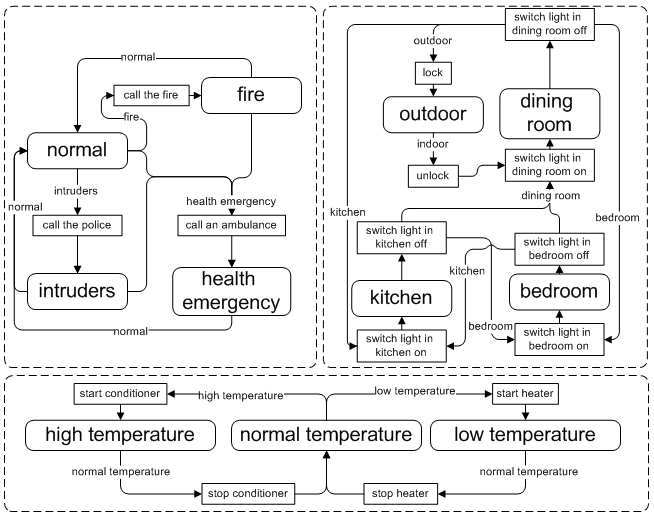
\includegraphics[width=\marginparwidth]{smarthome.png}
    \caption{Context diagram for Smart Home WSN.}
    \label{fig:cdsm}
  \end{figure}
}

Context can be defined as ``any information that can be used to characterize the situation of an entity, where an entity can be a person, place or physical object" \cite{dey99}. Using \textit{context} as a building block programmer could easily create an application for WSN, which is aware of changes in the environment.

Context-Oriented Programming \cite{hirschfeld08} is an approach which provides an opportunity for a programmer to develop a software which can dynamically change the behaviour depending on the activated context.

Thus, COP could be used as an effective way to use a \textit{Context} for developing a software for WSNs. It also will help to avoid the increasing complexity of a program. But bringing COP into WSNs is accompanied by following challenges.
\begin{itemize}\compresslist
\item
Context structure for WSNs could be very complex. In our example (Smart Home) there are a lot of possible \textit{contexts} like location in the specific room, climate states, levels of the light intensity etc. Some of \textit{contexts} are mutually exclusive, while other can be activated in parallel. For example, usually householder can't move from bathroom directly outside the house, thus this kind of the location change should be treated as an error. But climate state doesn't depend on the householder's location and corresponding \textit{contexts} can be activated or deactivated independently. Thus, there is a necessity to use a modified COP technique.
\item
Embedded platforms are mostly static, there are no tools for object-oriented or dynamic programming. Therefore, COP approaches for high-level languages (like Java, C++ or Python) are not applicable. 
\item
Embedded platforms also have restrictions on a hardware level, such as low memory, power consumption constraints, low CPU performance.
\end{itemize}

In this work we are proposing a COP technique for WSNs, which meets the challenges described above. Based on the concepts of the technique, which are described below, we developed a language called {\textlst{ConesC}} as a context-oriented extension of nesC language.

In {\textlst{ConesC}} we divided contexts into groups. It brings COP on a new level of abstraction and makes it possible to operate complex structures of contexts as a superposition of smaller substructures. Thus, every WSNs could have several mostly independent groups of contexts. Context transitions within the group are initiated by triggers and can be performed only if particular conditions are satisfied. There are also actions which should be performed before activation and after deactivation of the context.
% =============================================================================
\section{ConesC}
% =============================================================================
Figure \ref{fig:cdsm} shows a state diagram of possible contexts of \textit{Smart Home}. In this application two context groups could be found: \textit{Location} group and \textit{Temperature} group.

\paragraph{Householder's location.} WSN can track a householder's location. For example, if a householder moves from a bedroom to a dining room, the system switches off the light in the bedroom and switches on the light in the dining room. If a householder leaves the house, then \textit{Smart Home} could just lock the door. If a householder is nearby, then it could open the door.

\begin{Sbox}
\begin{minipage}{\marginparwidth}
\begin{csource}
(*@\textbf{context}@*) High {
(*@\lstnote{transitions}\textbf{transitions}@*) Normal;
(*@\lstnote{uses}@*)uses interface Leds;
}
implementation {
(*@\lstnote{activated}@*)event void activated(){}
(*@\lstnote{deactivated}@*)event void deactivated(){}
(*@\lstnote{check}@*)bool check(){return TRUE;}
(*@\lstnote{layeredimp}\textbf{layered}@*) void toggle_leds(){
  call Leds.set(1);
 }
}
\end{csource}
\end{minipage}
\end{Sbox}

\marginpar{
  \begin{figure}
    \TheSbox
    \caption{Context component.}
    \label{fig:cc}
  \end{figure}
}

\begin{Sbox}
\begin{minipage}{\marginparwidth}
\begin{csource}
(*@\textbf{context configuration}@*) Temperature {
(*@\lstnote{layereddef}\textbf{layered}@*) void toggle_leds();
}
implementation {
(*@\lstnote{contexts}\textbf{contexts}@*) High, 
(*@\lstnote{isdefault}@*) Normal (*@\textbf{is default}@*),
  Low;
 components LedsC;
 High.Leds -> LedsC;
 Normal.Leds -> LedsC;
 Low.Leds -> LedsC;
 Error.Leds -> LedsC;
}
\end{csource}
\end{minipage}
\end{Sbox}

\marginpar{
  \begin{figure}
    \TheSbox
    \caption{Context configuration component.}
    \label{fig:ccc}
  \end{figure}
}

\begin{Sbox}
\begin{minipage}{\marginparwidth}
\begin{csource}
(*@\lstnote{activate}\textbf{activate}@*) Temperature.High;
(*@\lstnote{call}@*)Temperature.toggle_leds();
\end{csource}
\end{minipage}
\end{Sbox}

\marginpar{
  \begin{figure}
    \TheSbox
    \caption{Usage example.}
    \label{fig:ue}
  \end{figure}
}

\paragraph{Climate control.} WSN can be programmed to detect specific conditions and activate a specific context. For example, if the temperature in the room is lower (or higher) than normal, system can enable air heating (or conditioning) to return the temperature to the normal state.


For demonstration purposes we are using TinyOS and nesC language, because it's a most popular tools for programming for WSNs. In order to use context-oriented paradigm, we added new key-words in the language. We are also extended components by \textit{context} and \textit{context configuration}. \textit{Context} is an analog of \textit{module} and \textit{context configuration} is an analog of \textit{configuration}. These two components can be used as other components in nesC language.

\textbf{Context} component is used to define context, possible transitions, actions before activation and after deactivation, layered functions, and to check transition conditions. In the rest it can be used like a \textit{module}.

On the figure \ref{fig:cc} context definition is displayed. Key word {\textlst{transitions}} on the line \lstref{transitions} define legal transitions from context \textit{High}. It means, that only \textit{Normal} can be activated as the next context after \textit{High}. This definition is not mandatory. If transitions are not defined, any transitions are legal. \nolinebreak

Line \lstref{uses} represents regular nesC key word and means, that we are using \textit{Leds} component. Event {\textlst{activated}} (line \lstref{activated}) is fired just before context activation, while event {\textlst{deactivated}} (line \lstref{deactivated}) is fired just after deactivation. These events are also not mandatory. Method {\textlst{check()}} on the line \lstref{check} is called to verify conditions of context activation. If {\textlst{check()}} returns {\textlst{FALSE}}, context will not be activated. If method is not defined, conditions will not be verified. Key-word {\textlst{layered}} (line \lstref{layeredimp}) indicates the implementation of the function, which is specific for the current context. The implementation of the \textit{layered} function is mandatory if it is defined in the context configuration.

\textbf{Context configuration} component is used to define layered functions and context configuration. In the rest it can be used like a regular \textit{configuration}.

In the listing \ref{fig:ccc} we assume, that contexts {\textlst{High}}, {\textlst{Normal}} and {\textlst{Low}} are already defined. {\textlst{Error}} context is default and generated by compiler, however it can be overridden by programmer in a standard context definition way. On the line \lstref{layereddef} we declare a layered function, which should be implemented in each context. Key-word {\textlst{contexts}} (line \lstref{contexts}) declares contexts, which are belonging to the \textit{Temperature} context group. It also indicates, that all declared contexts should implement layered functions. On the line \lstref{isdefault} context \textit{Normal} is declared as a context which will be active after initialization. The rest of the listing is a regular declaration of components and wires.

{\textlst{Context}} and {\textlst{context configuration}} have nesC-like structure and utilize the same logic. Both components can be used in native nesC way as a regular components.

\balance
\bibliographystyle{acm-sigchi}
\bibliography{ubicomp}

\end{document}
